\documentclass[a4paper,11pt]{jsarticle}

\usepackage[dvipdfmx]{graphicx}
\usepackage[hang,small,bf]{caption}
\usepackage[subrefformat=parens]{subcaption}
\captionsetup{compatibility=false}

\begin{document}
  \begin{figure}[htbp]
    \centering
    \begin{minipage}{0.45\linewidth}
      \centering
      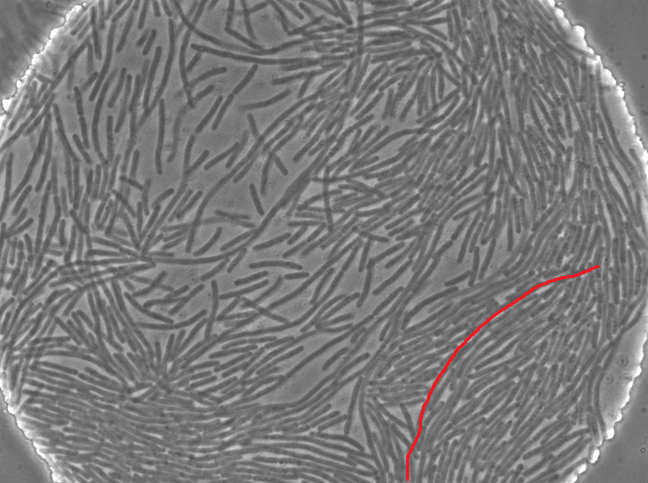
\includegraphics[width=\columnwidth]{Series015_t090000_RAW_ch00.png}
      \subcaption{菌液注入から約後}
      \label{fig:06_1_pt}
    \end{minipage}
    \begin{minipage}{0.45\linewidth}
      \centering
      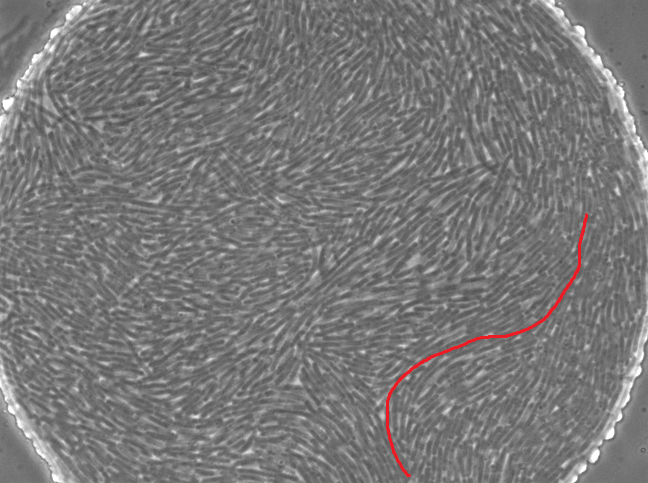
\includegraphics[width=\columnwidth]{Series015_t120000_RAW_ch00.png}
      \subcaption{菌液注入から約後}
      \label{fig:06_2_pt}
    \end{minipage}
    \begin{minipage}{0.45\linewidth}
      \centering
      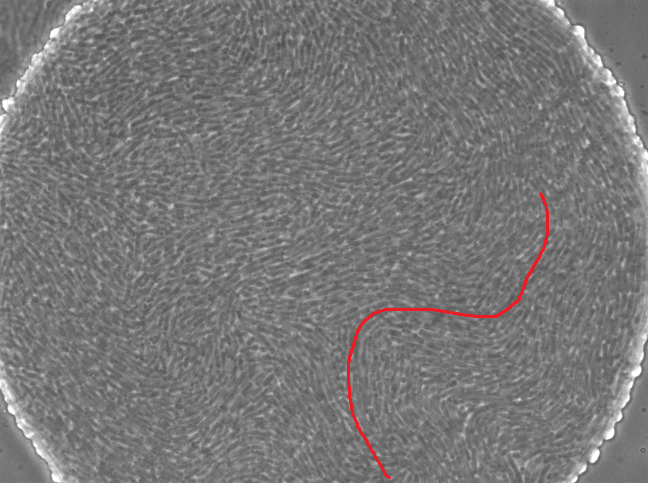
\includegraphics[width=\columnwidth]{Series015_t150000_RAW_ch00.png}
      \subcaption{菌液注入から約後}
      \label{fig:06_3_pt}
    \end{minipage}
    \begin{minipage}{0.45\linewidth}
      \centering
      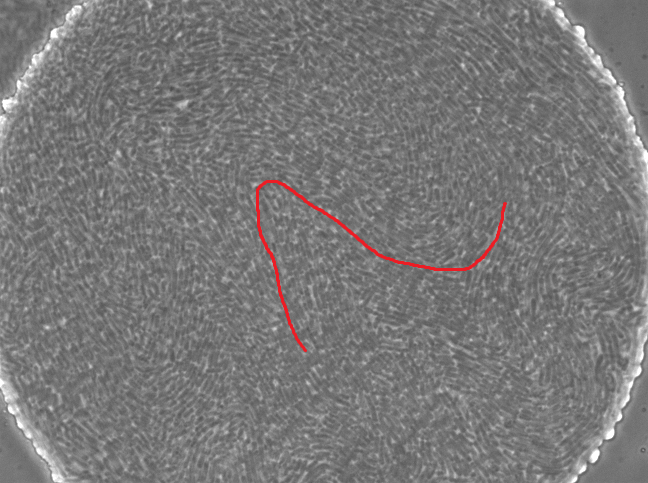
\includegraphics[width=\columnwidth]{Series015_t180000_RAW_ch00.png}
      \subcaption{菌液注入から約後}
      \label{fig:06_4_pt}
    \end{minipage}
    \caption{UU2806を用いた実験の結果.繊維状の個体に対応する場所を赤くマークした.}
  \end{figure}
  \end{document}
